\section{Twitter}
Twitter is a real-time information network that connects you to the latest stories, ideas, opinions and news about what you find interesting. All information on Twitter is distributed through ``tweets'', small 140-character messages where a person can shortly state an opinion, an event or random thoughts. Because of the format, twitter encourages frequent updates from users and as of October 26th, 2012 around 500 million tweets are written per day (24 hours)\cite{Cnet1}. With 140 million users, this means each user, on average, posts 3.5 tweets per day. A typical tweet can be seen below.
\newline
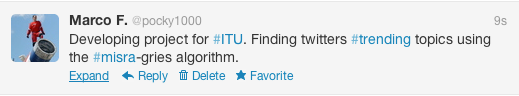
\includegraphics[width=125mm]{tweet.png}
\newline

Each user on twitter chooses other users to follow and see an aggregated list of all their tweets. Tweets can be replied to by in this form:

\begin{quote}
    @pocky1000 You are totally right. \#ITU is super cool.
\end{quote}

\subsection{Hashtags and topics}
For the purpose of categorizing tweets, users put hashtags within their tweets. Examples include, as seen above, \#ITU, \#trending and \#Misra. For the purpose of this paper, we will consider these hashtags as topics, and will only consider tweets that contain at least one hashtag. If a tweet contains several hashtags, it will add to our counter for each of them seperately. It will also be used individually for each one when considering uniqueness (so it might be unique to one hashtag but not to another).

Users of twitter can see the tweets of people they follow, and have the options to either reply to a tweet, or retweet it. On retweet the user basically shares the same message to their own followers, giving credit to the creator of the message.
The topic of a tweet is identified by the presence of a hashtag \# in front of a word. In the example above the topics are \#ITU,\#trending and \#Misra.
Tweets can be tagged by writing a hashtag ``\#'' followed by a topic or keyword. Twitter users this as a way to categorize messages.
A trending topic is defined by a topic that has a high frequency, in other words many people are ``tweeting'' about the same topic at some point in time. A trending topic can either be many unique tweets about the same topic, e.g. if people are tweeting to promote some beneficial cause, or it can be the same message retweeted by many users.
Twitter currently have over 500 million users, so the amount of tweets produced at any moment is equally big, some specifics. We use the public Twitter API to create a stream of which corresponds to a sample of all tweets. 